\documentclass[11pt]{article}
\usepackage[pdftex]{graphicx}
\usepackage[explicit]{titlesec}
\usepackage[OT1]{fontenc}
\usepackage[most]{tcolorbox}
\usepackage[final]{pdfpages}
\usepackage[colorlinks=true, urlcolor=cyan, hyperfootnotes=false]{hyperref}
\usepackage{fullpage, graphicx, psfrag, url, caption, authblk, amsfonts, amsmath, amssymb, float, fancyhdr, multicol, cmbright, xcolor, amsthm, gensymb, physics}

\fancypagestyle{pages}{
	%Headers
	\fancyhead[L]{Physics 7A, Summer 2024 \\ Section 103}
	%\fancyhead[C]{\thepage}
	\fancyhead[R]{Discussion 4 \\ June 24}
\renewcommand{\headrulewidth}{0pt}
	%Footers
	%\fancyfoot[L]{}
	\fancyfoot[C]{}
	\fancyfoot[R]{\thepage}
\renewcommand{\footrulewidth}{0pt}
}

\newcommand\blfootnote[1]{
    \begingroup
    \renewcommand\thefootnote{}\footnote{#1}
    \addtocounter{footnote}{-1}
    \endgroup
}

\newcommand{\fig}[4]{
    \begin{figure}[H]
        \centering
        \includegraphics[scale={#3}, angle={#4}]{#1}
        \caption{#2}
        \label{exp4fit}
    \end{figure}
}

\newtheoremstyle{gangnamstyle}{}{}{}{}{\sffamily\bfseries}{.}{ }{}
\tcolorboxenvironment{definition}{boxrule=0pt,boxsep=0pt,colback={blue!10},left=8pt,right=8pt,enhanced jigsaw, borderline west={2pt}{0pt}{blue},sharp corners,before skip=10pt,after skip=10pt,breakable}
\tcolorboxenvironment{example}{boxrule=0pt,boxsep=0pt,colback={orange!10},left=8pt,right=8pt,enhanced jigsaw, borderline west={2pt}{0pt}{orange},sharp corners,before skip=10pt,after skip=10pt,breakable}
\tcolorboxenvironment{problem}{boxrule=0pt,boxsep=0pt,colback={cyan!10},left=8pt,right=8pt,enhanced jigsaw, borderline west={2pt}{0pt}{cyan},sharp corners,before skip=10pt,after skip=10pt,breakable}
\theoremstyle{gangnamstyle}{\newtheorem{definition}{Definition}[]}
\theoremstyle{gangnamstyle}{\newtheorem{example}{Example}[]}
\theoremstyle{gangnamstyle}{\newtheorem{problem}{Problem}[]}

\headheight=0pt
\footskip=0pt
\setlength{\oddsidemargin}{0 in}
\setlength{\evensidemargin}{0 in}
\setlength{\topmargin}{-0.5 in}
\setlength{\textwidth}{6.5 in}
\setlength{\textheight}{8.5 in}
\setlength{\headsep}{0.75 in}
\setlength{\parindent}{0 in}
\setlength{\parskip}{0.1 in}

\begin{document}
\normalfont
\pagestyle{pages}

% Begin Document

\begin{center}
\vspace{3in}
{\Large Discussion 4 } \\ [0.05in]
Projectile Motion \\ [-0.5in]
\end{center}

\section*{Topics}
Uniform Acceleration in 2D, Projectile Motion

\section{Review}

\begin{itemize}
\item We can apply all the arguments we have learned about kinematics to solve for 2D Projectile motion. In particular, an object under free fall has uniform acceleration in the $y$-direction, and no acceleration in the $x$-direction. 
\[ \Vec{a} = 0\Hat{x} - g\Hat{y} \]

\item $x$-direction:
\[ a_x = 0 \]
\[ v_x = v_{0x} \]
\[ x = x_0 + v_x t \]

\item $y$-direction:
\[ a_y = -g \]
\[ v_y = v_{0y} + a_yt \]
\[ y = y_0 + v_{0y}t + \frac{1}{2}a_yt^2 \]
\[ v_y^2 = v_{0y}^2 + 2a_y(y - y_0) \]

\item Typically, the time of flight $t$ is determined by the motion in the $y$-direction, from the time the projectile is launched until it hits the ground. In turn, this $t$ affects the range $R$ traveled in the $x$-direction. 

\end{itemize}

\pagebreak

\section{Projectile Motion}

\textbf{1.} \textit{Giancoli, Physics for Scientists and Engineers, Problem 3.51} \\
A ball is thrown horizontally from the top of a cliff with initial speed $v_0$ (at $t = 0$). At any moment, its direction of motion makes an angle $\theta$ to the horizontal. Derive a formula for $\theta$ as a function of time as the ball follows a projectile’s path. 
\fig{figs/0620/proj.png}{Giancoli, Problem 3.51}{0.75}{0}
\vspace{2 in}

\textbf{2.} \textit{Morin, Introduction to Classical Mechanics, Exercise 2.13} \\
A ball is dropped from height $4h$. After it has fallen a distance $d$, a second ball is dropped from height $h$. What should d be (in terms of $h$) so that the balls hit the ground at the same time?

\vspace{2 in}

\textbf{3.} \textit{Morin, Introduction to Classical Mechanics, Exercise 2.19} \\
Two balls are fired from ground level, a distance $d$ apart. The right one is
fired vertically with speed $v$, see Fig 2.20. You wish to simultaneously fire the left one at the appropriate velocity $\Vec{u}$ so that it collides with the right ball when they reach their highest point. What should $\Vec{u}$ be (give the horizontal and vertical components)? Given $d$, what should $v$ be so that the speed $u$ is minimum?
\fig{figs/0624/morin219.png}{Morin, Exercise 2.19}{0.75}{0}
\vspace{1 in}


\textbf{4.} \textit{Giancoli, Physics for Scientists and Engineers, Problem 3.61} \\
Derive a formula for the horizontal range $R$ of a projectile when it lands at a height $h$ above its initial point. (For $h < 0$, it lands a distance $-h$ below the starting point.) Assume it is projected at an angle $\theta_0$ with initial speed $v_0$.
\fig{figs/0624/giancoli361.png}{Giancoli, Problem 3.61}{0.75}{0}
\textit{Hint: The Quadratic Formula:} $ax^2 + bx + c = 0 \implies x = \frac{-b \pm \sqrt{b^2 - 4ac}}{2a}$. \\
\vspace{3 in}

\textbf{5.} \textit{Giancoli, Physics for Scientists and Engineers, Problem 3.60} \\
A person stands at the base of a hill that is a straight incline making an angle $\phi$ with the horizontal. For a given initial speed $v_0$, at what angle $\theta$ (to the horizontal) should objects be thrown so that the distance $d$ they land up the hill is as large as possible?
\fig{figs/0624/giancoli360.png}{Giancoli, Problem 3.60}{0.75}{0}
\textit{Hint:} \\
$\arctan(-\cot(\phi)) = \phi - \frac{\pi}{2}$. \\
$\arctan(\phi) = \arctan(\phi) + \pi$. This sounds weird mathematically, but if you take the $\tan$ of both sides, they are indeed equal. Intuitively, $\theta$ should be a positive quantity. If you arrive at a negative answer, you should add a $\pi$ to it. 
\vspace{2 in}

\textbf{6-8.} \textit{Problems from 7A Workbook and Past Exams (Next Pages)}
\vspace{1 in}

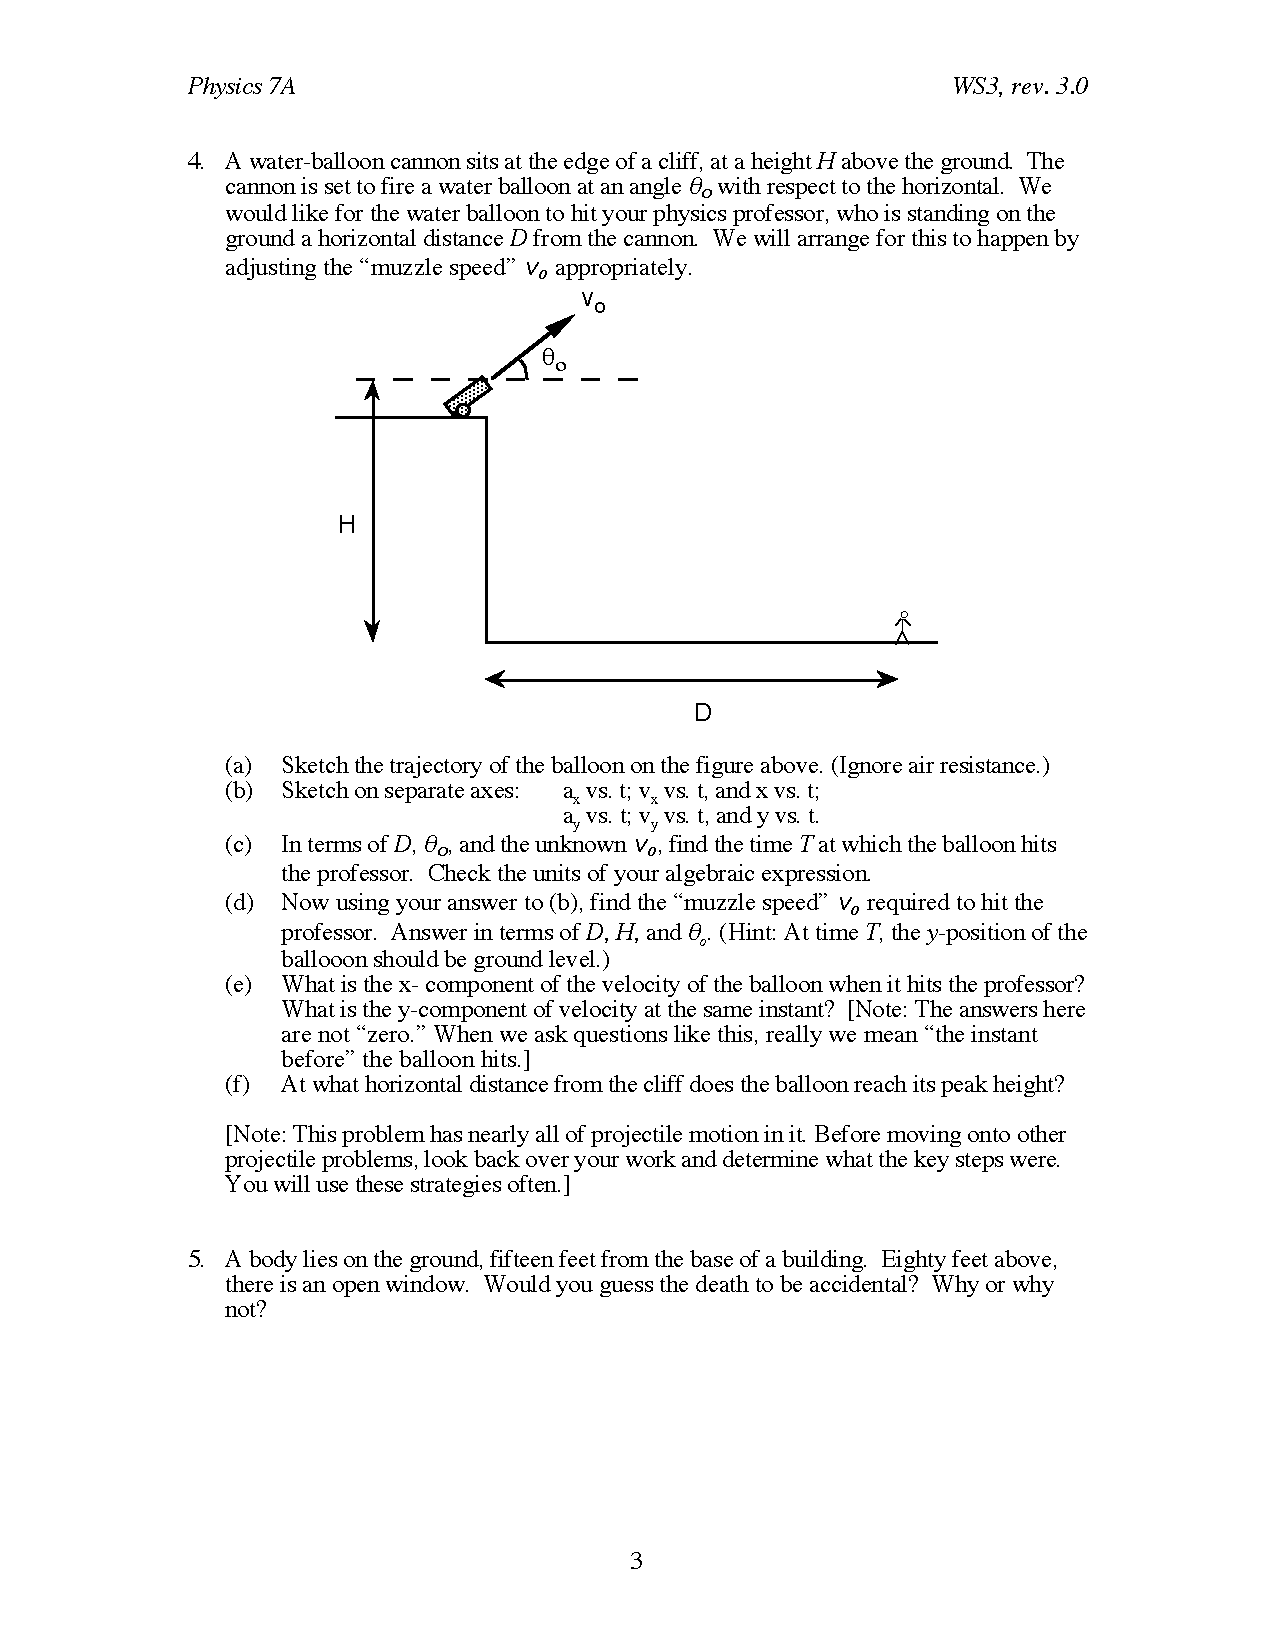
\includepdf[pages=-]{figs/0620/wb19.pdf}

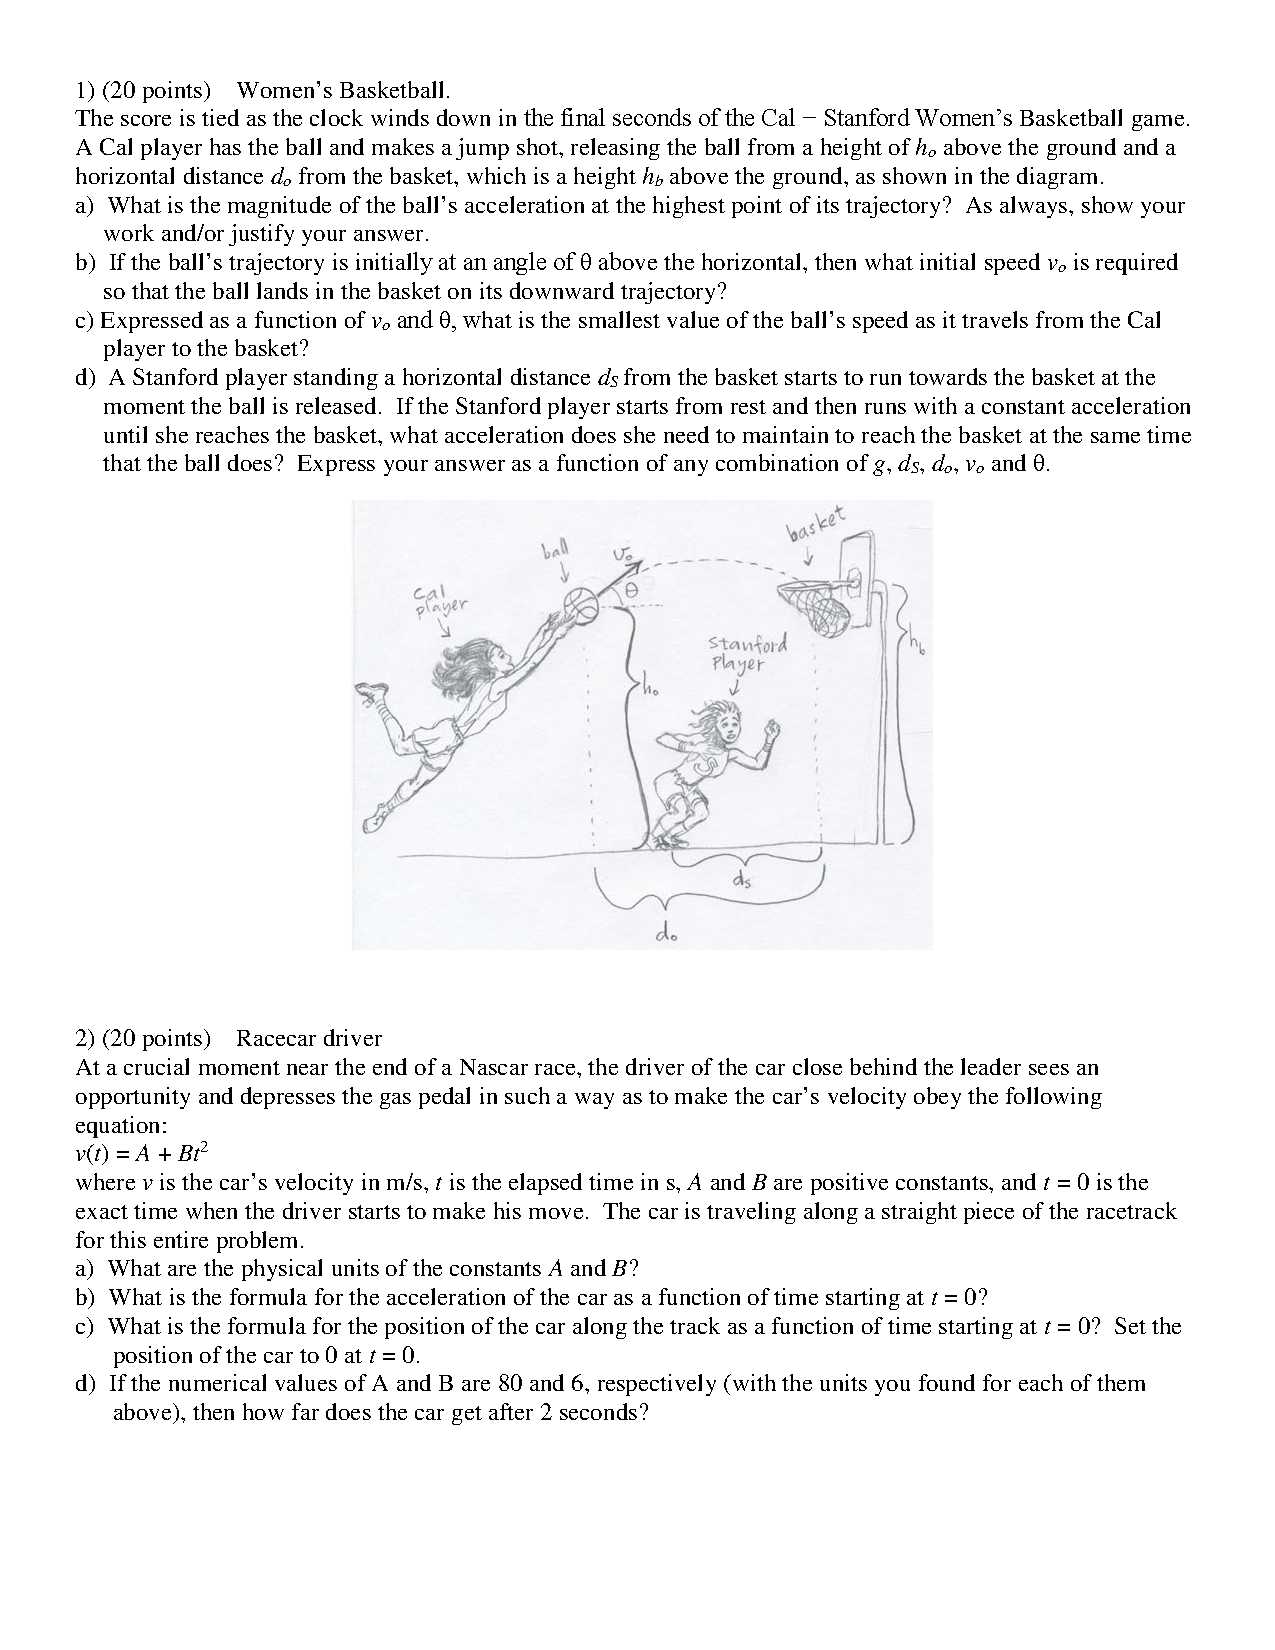
\includepdf[pages=-]{figs/0620/mt14.pdf}

\end{document}
